\documentclass{article}
\usepackage{tikz}
\usepackage{layout}
\usepackage{pgfmath}

\usetikzlibrary{intersections}
\usetikzlibrary{calc}

\tikzset{help lines/.style={very thin}}

\tikzset{help lines rojo1/.style={help lines,color=red!25}}
\tikzset{help lines rojo2/.style={help lines,color=red!50}}
\tikzset{help lines rojo3/.style={help lines,color=red!75}}
\tikzset{help lines rojo4/.style={help lines,color=red!90}}

\tikzset{Alex's grid/.style={help lines,color=#1!50,step=.5cm},
		 Alex's grid/.default=blue}

\begin{document}
	\tikz \draw [thick, rounded corners=8pt] (0,0) -- (0,2) -- (1,3.25) -- 
		(2,2) -- (2,0) -- (0,2) -- (2,2) -- (0,0) -- (2,0);\\[10pt]

We are working on
\begin{tikzpicture}
	\draw (-1.5,0) -- (1.5,0);	%	one unit is one cm.
	\draw (0,-1.5) -- (0,1.5);
	\draw (-1,0) .. controls (-1,0.555) and (-0.555,1) .. (0,1);
	\draw (0,1)  .. controls (0.555,1)  and (1,0.555)  .. (1,0);
\end{tikzpicture}.\\[50pt]
	\tikz{\draw (-1,-2) -- (.5,.3)}\\[50pt]
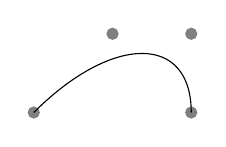
\begin{tikzpicture}
	\filldraw [gray] 	(0,0) circle (2pt)
						(1,1) circle (2pt)
						(2,1) circle (2pt)
						(2,0) circle (2pt);
	\draw (0,0) .. controls (1,1) and (2,1) .. (2,0);
\end{tikzpicture}\\[50pt]
\tikz \draw (0,0) circle (10pt);
\tikz \draw (0,0) ellipse (15pt and 10pt);
\tikz \draw [rotate=30] (0,0) ellipse (5pt and 3pt);
\\[50pt] 
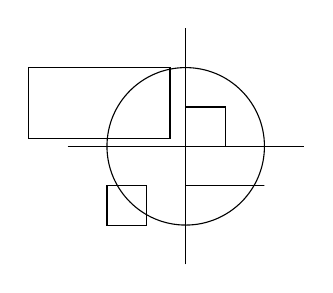
\begin{tikzpicture}
	\draw (-1.5,0) -- (1.5,0);	%	one unit is one cm.
	\draw (0,-1.5) -- (0,1.5);
	\draw (0,0) circle (1cm);
	\draw (0,0) rectangle (.5,.5);
	\draw (-.5,-.5) rectangle (-1,-1);
	\draw (0,-.5) rectangle (1,-.5);
	\draw (-2,1) rectangle (-.2,.1);
\end{tikzpicture}
\\[30pt]
The code \verb+\tikz \draw[step=2pt] (0,0) grid (10pt,10pt);+ produces \tikz \draw[step=2pt] (0,0) grid (10pt,10pt);.\\[15pt]
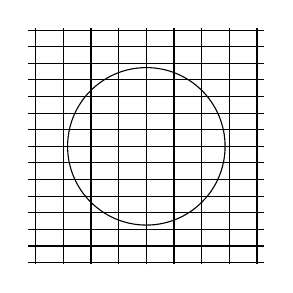
\begin{tikzpicture}%si no da divisible no lo cierra
	\draw (-1.5,0) -- (1.5,0);	
	\draw (0,-1.5) -- (0,1.5);
	\draw (0,0) circle (1cm);
	\draw[xstep=10pt,ystep=6pt] (-1.5,-1.5) grid (1.5,1.5);
\end{tikzpicture}\\[15pt]
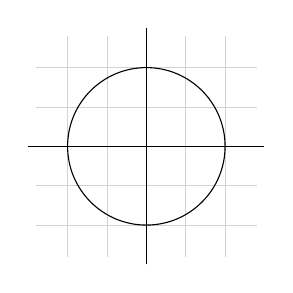
\begin{tikzpicture}
	\draw[step=.5cm,help lines rojo1] (-1.4,-1.4) grid (1.4,1.4);
	\draw (-1.5,0) -- (1.5,0);
	\draw (0,-1.5) -- (0,1.5);
	\draw (0,0) circle (1cm);
\end{tikzpicture}
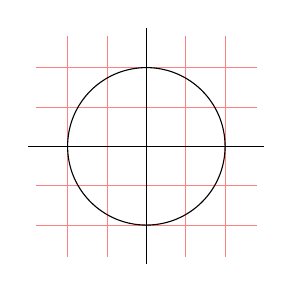
\begin{tikzpicture}
	\draw[step=.5cm,help lines rojo2] (-1.4,-1.4) grid (1.4,1.4);
	\draw (-1.5,0) -- (1.5,0);
	\draw (0,-1.5) -- (0,1.5);
	\draw (0,0) circle (1cm);
\end{tikzpicture}
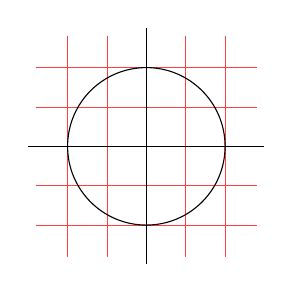
\begin{tikzpicture}
	\draw[step=.5cm,help lines rojo3] (-1.4,-1.4) grid (1.4,1.4);
	\draw (-1.5,0) -- (1.5,0);
	\draw (0,-1.5) -- (0,1.5);
	\draw (0,0) circle (1cm);
\end{tikzpicture}
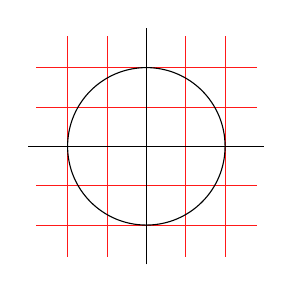
\begin{tikzpicture}
	\draw[step=.5cm,help lines rojo4] (-1.4,-1.4) grid (1.4,1.4);
	\draw (-1.5,0) -- (1.5,0);
	\draw (0,-1.5) -- (0,1.5);
	\draw (0,0) circle (1cm);
\end{tikzpicture}\\[15pt]
\begin{tikzpicture}
	\draw[loosely dashed] 	(-2,1) rectangle (-.2,.1);
	\draw[dashed] 			(.5,1) rectangle +(1.8,-0.9);
	\draw[loosely dotted] 	(3,1)  rectangle (4.8,.1);
	\draw[dotted] 			(5.5,1) rectangle (7.3,.1);
\end{tikzpicture}\\[15pt]
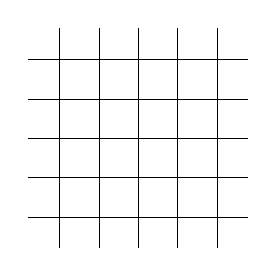
\begin{tikzpicture}
	\draw[color=black,step=.5cm,ultra thin] (-1.4,-1.4) grid (1.4,1.4);
\end{tikzpicture}
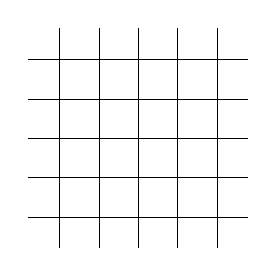
\begin{tikzpicture}
	\draw[color=black,step=.5cm,very thin] (-1.4,-1.4) grid (1.4,1.4);
\end{tikzpicture}
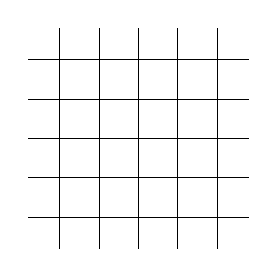
\begin{tikzpicture}
	\draw[color=black,step=.5cm,thin] (-1.4,-1.4) grid (1.4,1.4);
\end{tikzpicture}
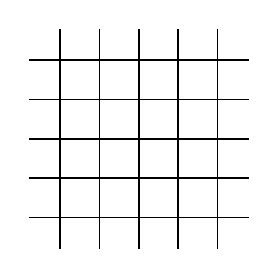
\begin{tikzpicture}
	\draw[color=black,step=.5cm,semithick] (-1.4,-1.4) grid (1.4,1.4);
\end{tikzpicture}
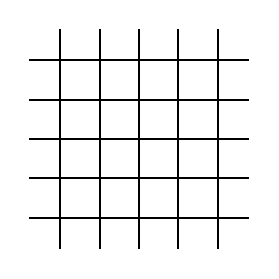
\begin{tikzpicture}
	\draw[color=black,step=.5cm,thick] (-1.4,-1.4) grid (1.4,1.4);
\end{tikzpicture}
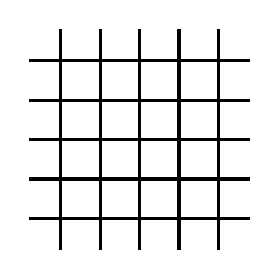
\begin{tikzpicture}
	\draw[color=black,step=.5cm,very thick] (-1.4,-1.4) grid (1.4,1.4);
\end{tikzpicture}
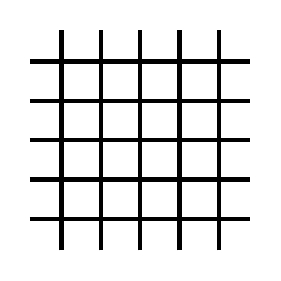
\begin{tikzpicture}
	\draw[color=black,step=.5cm,ultra thick] (-1.4,-1.4) grid (1.4,1.4);
\end{tikzpicture}
\\[15pt]
\begin{tikzpicture}
	\draw[Alex's grid=black] (2.6,-1.4) grid (5.4,1.4);
	\draw (0,0) arc (0:315:1.75cm and 1cm);
\end{tikzpicture}
\\[15pt]
\tikz \draw[Alex's grid] 	(0,0) grid (2,4)
							(0,0) rectangle (2,4)
							(0,0) parabola (2,4); Con dos puntos alcanza
							para interpolar \emph{media} par\'abola.
\tikz \draw[x=1ex,y=1ex] (0,0) sin (1.57,1);\\[10pt]
Ahora con unidades de $\pi/2$!:
\tikz \draw[x=1.57cm,y=1cm] (0,0) sin (1,1) cos (2,0) sin (3,-1) cos (4,0)
							(0,1) cos (1,0) sin (2,-1) cos (3,0) sin (4,1);
\\[15pt]
Por qu\'e conviene usar \verb+cycle+:
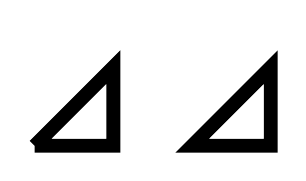
\begin{tikzpicture}[line width=5pt]
	\draw (0,0) -- (1,0) -- (1,1) -- (0,0);
	\draw (2,0) -- (3,0) -- (3,1) -- cycle;
	\useasboundingbox (0,1.5);
\end{tikzpicture}
\\[15pt]

\begin{tikzpicture}
	\shadedraw[draw=yellow,fill=black,rounded corners,
				left color=yellow,right color=black] (0,0) rectangle +(3,2);
	\shade[rounded corners,outer color=black,inner color=yellow]
		(4,0) rectangle +(3,2);
\end{tikzpicture}
\\[15pt]
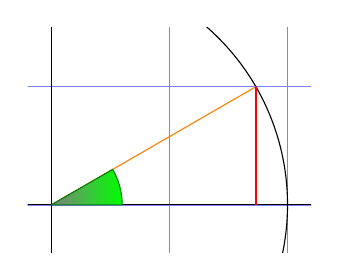
\begin{tikzpicture}[scale=3]
	\clip (-0.1,-0.2) rectangle (1.1,0.75);
	\draw[Alex's grid] (-1.4,-1.4) grid (1.4,1.4);
	\draw (-1.5,0) -- (1.5,0);
	\draw (0,-1.5) -- (0,1.5);
	\draw (0,0) circle (1cm);
	\draw[thin,orange] (0,0) -- (30:1cm);
	\shadedraw[left color=gray,right color=green,draw=green!50!black]
		(0,0) -- (3mm,0) arc (0:30:3mm) -- cycle;
	\draw[thick,red] (30:1) -- (30:1cm |- 0,0); % intersecciones
\end{tikzpicture}
\\[15pt]
To appreciate the difference between + and ++\\[15pt]
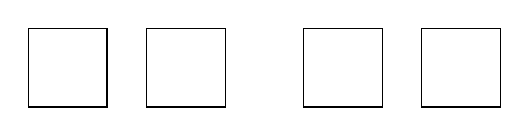
\begin{tikzpicture}
	\def\rectanglepath{-- ++(1cm,0cm) -- ++(0cm,1cm)
					   -- ++(-1cm,0cm) -- cycle}
	\draw (0,0) \rectanglepath;
	\draw (1.5,0) \rectanglepath;

	\def\rectanglepathBis{-- +(1cm,0cm) -- +(1cm,1cm) -- +(0,1) -- cycle}
	\draw (3.5,0) \rectanglepathBis;
	\draw (5,0) \rectanglepathBis;
\end{tikzpicture}
\\[15pt]
\begin{tikzpicture}
	\draw[<->] (0,0) arc (0:180:2);
	\draw[->] (1,0) -- (2,1) -- (3,0) -- (4,1); %% ??
	\draw[->] (1,0) -- (1.5cm,10pt) -- (2cm,0pt) -- (2.5cm,10pt);\\
	\draw[<->>, >=stealth] (5,0) arc (0:38:1);
\end{tikzpicture}
\\[15pt]
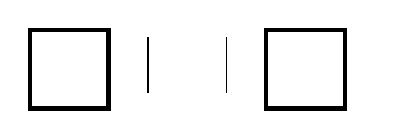
\begin{tikzpicture}[ultra thick]
	\draw (0,0) rectangle +(1,1);
	\begin{scope}[thin]
		\clip (1.4,0.2) rectangle +(3.1,0.7);  % el clip se restringe al scope 
		\draw (1.5,0) rectangle +(1,1);
	\end{scope}
	\draw (3,0) rectangle +(1,1);
\end{tikzpicture}
\\[15pt]
\begin{tikzpicture}
	\draw (-3,2) [thin] -- (-0.7,0.3) -- (1.23,.5) [thick];
\end{tikzpicture}
\\[15pt]
\tikz \draw (0,0) -- (0,0.5) [xshift=5pt] (0,0) -- (0,0.5);
\\[15pt]
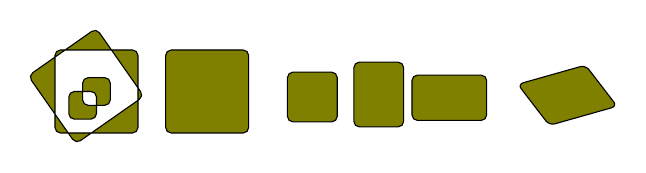
\begin{tikzpicture}[even odd rule,rounded corners=2pt,x=10pt,y=10pt]
	\def\examplefill{green!50!red}  % aplica desde el lugar en adelante!
	\filldraw[fill=\examplefill] (0,0) rectangle (1,1)
		[xshift=5pt,yshift=5pt]  (0,0) rectangle (1,1)
		 			 			 (-1,-1) rectangle (2,2)
		[rotate=35] 			 (-1,-1) rectangle (2,2)
		[rotate=-35,shift={(4,0)}] (-1,-1) rectangle (2,2)
		[shift={+(2,-2)},scale=.6]		 (-1,-1) rectangle (2,2)
		[shift={+(2,-2)},yscale=1.3]		 (-1,-1) rectangle (2,2)
		[shift={+(2,-2)},xscale=1.5,yscale=0.7]		 (-1,-1) rectangle (2,2)
		[shift={+(3,-2)},rotate=25]		 (-1,-1) rectangle (2,2);
\end{tikzpicture}
\\[15pt]
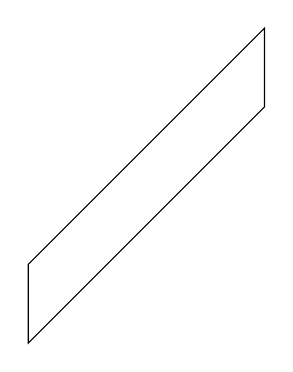
\begin{tikzpicture}
	\draw[yslant=1] (0,0) rectangle (3,1);
\end{tikzpicture}
\\[15pt]
\tikz \foreach \x in {1,2,3} {$x=\x, $};
\\[15pt]
\tikz \foreach \x in {1,...,10} {\filldraw[fill=orange,draw=green] (.33*\x,{.25*pow(\x*.33,1.8)}) circle (3pt);};
\\[15pt]
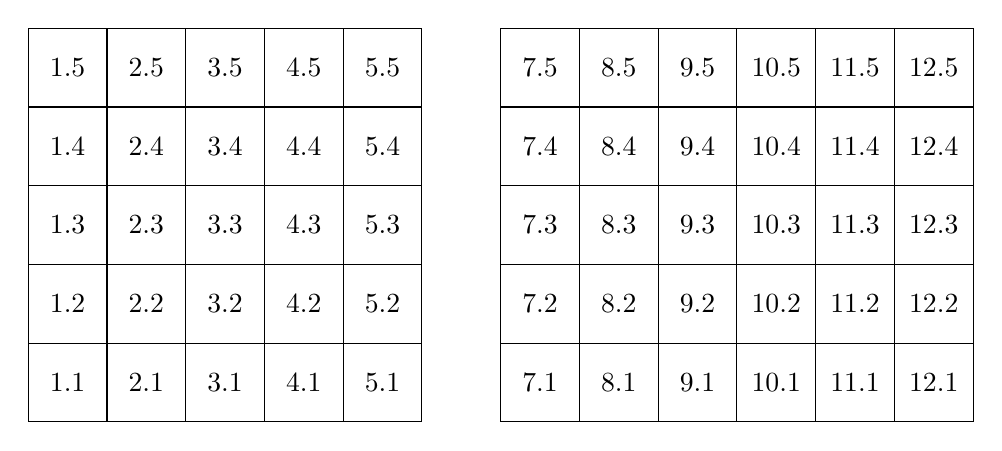
\begin{tikzpicture}
	\foreach \x in {1,2,...,5,7,8,...,12}
		\foreach \y in {1,...,5}
		{
			\draw (\x,\y) +(-.5,-.5) rectangle +(.5,.5);
			\draw (\x,\y) node{\x.\y};
		}
\end{tikzpicture}
\\[15pt]
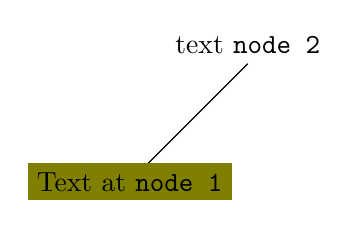
\begin{tikzpicture}
	\draw (-.5,-.5) node[fill=red!50!green] {Text at \verb!node 1!} --
			(1,1) node[anchor=south] {text \verb+node 2+};
\end{tikzpicture}
\\[15pt]
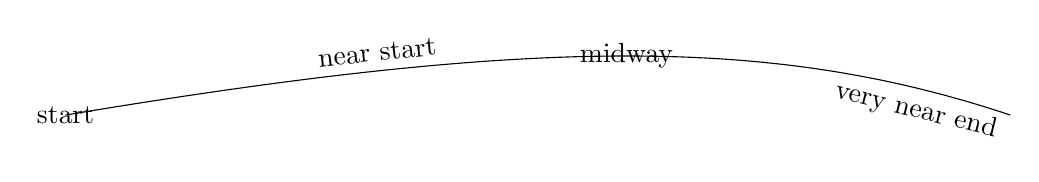
\begin{tikzpicture}
	\draw (0,0) node[sloped] {start} .. controls (6,1) and (9,1) .. 
		node[near start,sloped,above] 	{near start}
		node[midway]					{midway}
		node[very near end,sloped,below]{very near end} (12,0);
\end{tikzpicture}
\\[15pt]
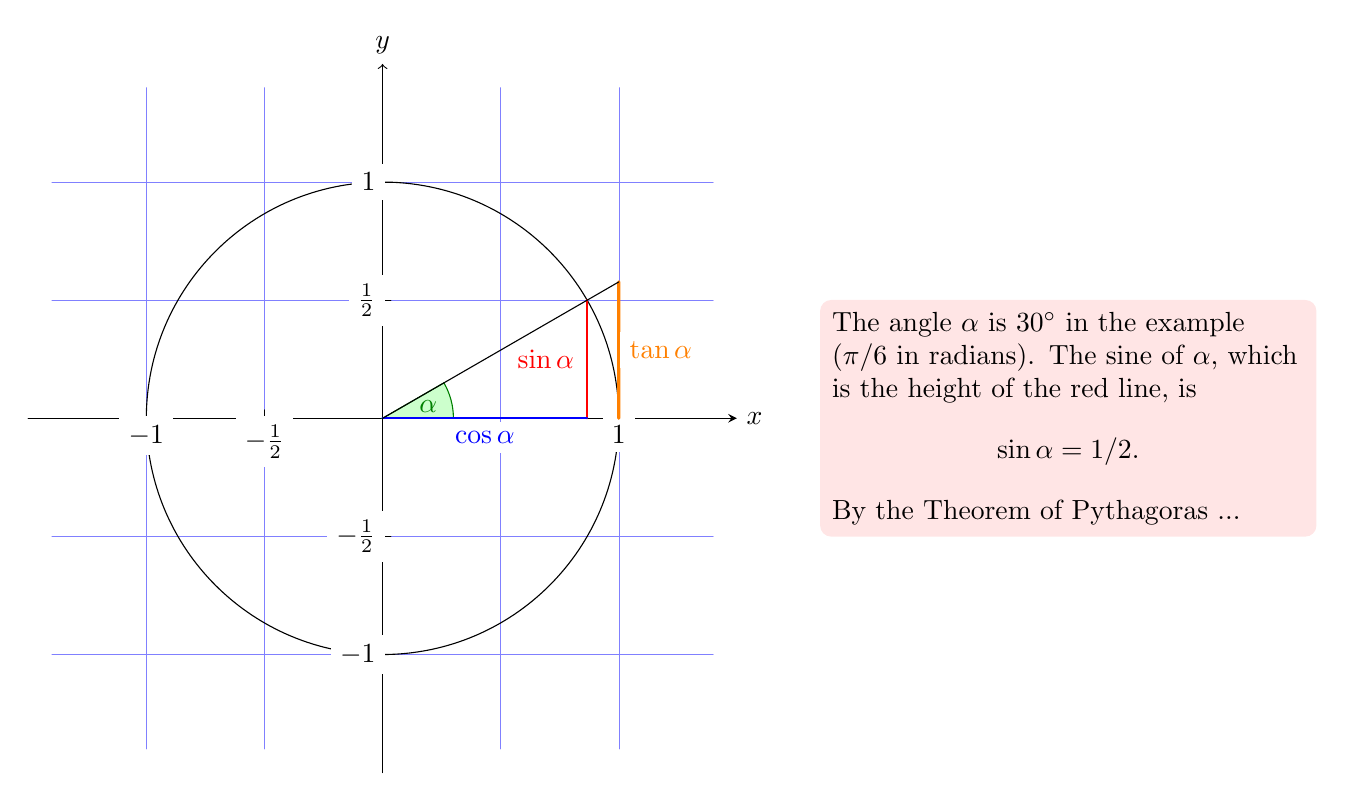
\begin{tikzpicture}[scale=3,line cap=round,axes/.style=]
	%\clip (-0.1,-0.2) rectangle (1.1,0.75);
	\draw[Alex's grid] (-1.4,-1.4) grid (1.4,1.4);

	\draw (0,0) circle (1cm);

	\begin{scope}[axes]
		\draw[->,>=stealth] (-1.5,0) -- (1.5,0) node[right] {$x$};
		\draw[->,] (0,-1.5) -- (0,1.5) node[above] {$y$};
		\foreach \x/\xtext in {-1,-.5/-\frac{1}{2},1}    % h = diferencia de los primeros dos
			\draw (\x,-1pt) -- (\x,1pt) node[below=2pt,fill=white] {$\xtext$};
		\foreach \x/\xtext in {-1,-.5/-\frac{1}{2},.5/\frac{1}{2},1}    % h = diferencia de los primeros dos
			\draw (-1pt,\x) -- (1pt,\x) node[left=2pt,fill=white] {$\xtext$};
	\end{scope}	

	\filldraw[fill=green!20!white,draw=green!50!black]
		(0,0) -- (3mm,0) arc (0:30:3mm) -- cycle;
	\draw (15:2mm) node[green!50!black] {$\alpha$};
	
	\draw[thick,red] 
		(30:1cm) -- node[left=1pt,fill=white] {$\sin\alpha$} +(0,-0.5);
	
	\draw[thick,blue] 
		(30:1cm) ++(0,-.5) -- node[below=1pt,fill=white] {$\cos\alpha$} (0,0);
	\path[name path=vertical] (1,0) -- (1,1);
	\path[name path=pendiente] (0,0) -- (30:1.5cm);
	\draw[name intersections={of=pendiente and vertical, by=x}]
		[orange, very thick] (1,0) -- node[right,fill=white] 
		{$\tan\alpha$} (x);

	\draw (0,0) -- (x);

	\draw[xshift=1.85cm] (0,0) 
		node[right,rounded corners,fill=red!10,inner sep=1ex,text width=6cm]
		{
			The angle $\alpha$ is $30^\circ$ in the
			example ($\pi/6$ in radians). The sine of
			$\alpha$, which is the height of the red line, is
			\[
				\sin \alpha = 1/2.
			\]
			By the Theorem of Pythagoras ...
		};
\end{tikzpicture}
\end{document}